\chapter{Background}
\vspace{-1pc}
Virtual reality gets integrated into everyday life closer and closer.
Regarding Augmented Reality, it considered as an enhanced version of human eye view, where visualisation on the real world gets modified by new technologies~\cite{reality_tech_what_2018}.
The purpose of this project is to follow that flow and introduce the advantages of Mixed Reality to establish new boundaries and goals for people to reach.
By creating a framework of a realistic mixed reality within Tank Commander Game, the project investigates the limits of current technological progress over the first part of the research, implements the discussed techniques over the second and sets new goals to extend further at the end.
As a result, the overall goal of the project is to demonstrate how Mixed Reality (MR) can be used to establish a new concept, which humanity may go more in-depth in improving Virtual worlds by bringing some pieces of the real one and wherefore discovering advantages and possibilities to improve human perception within Augmented.
On top of that, it comes up with new issue and difficulties, which some of them got appropriately considered and resolved, another left for future researches to implement.\\[1pt]
Currently, the project consists of several hardware and software components. $1/16^{th}$ remote control tank model, which run by a Small Portable Computer(SPB) Raspberry Pi 3 (R-Pi)~\cite{raspberrypi_raspberry_2019}, $360\circ$ camera, and raw close-quarter testing arena.
The scene gets linked to HTC VR gear set~\cite{vive_vive_2019}, which recreates Software Components with Unity Game Engine and SteamVR support. \\
Finally, the FFmpeg~\cite{fate_ffmpeg_2018} - open-source library to manage and process the upcoming video stream and TensorFlow as a base for complicated computations on a Graphical Card (GPU). 
GPU is powered by NVIDIA CUDA cores to allow maximum performance in video processing and, therefore, eliminate any unfortunate lags.
The game engine defines the rest of the gameplay details.
Raspberry-Pis' (R-Pi) primary goal is to control motors inside a toy tank, which is responsible for wheel rotation and direction as well as the position of the gun.
However, the Wireless Communication feature allows to set up a python based socket server, which will receive commands from any other devices within the same network.
Commands or Control operations performed inside Unity will be sent to R-Pi and mirror most of the actions a similar virtual tank performs.
FFMPEG library, which was used mostly for converting video stream into texture material inside Unity, now performs an additional role, by capturing and restreaming video forward.
\begin{figure}[H]
	\centering
	\begin{subfigure}[b]{0.4\textwidth}
		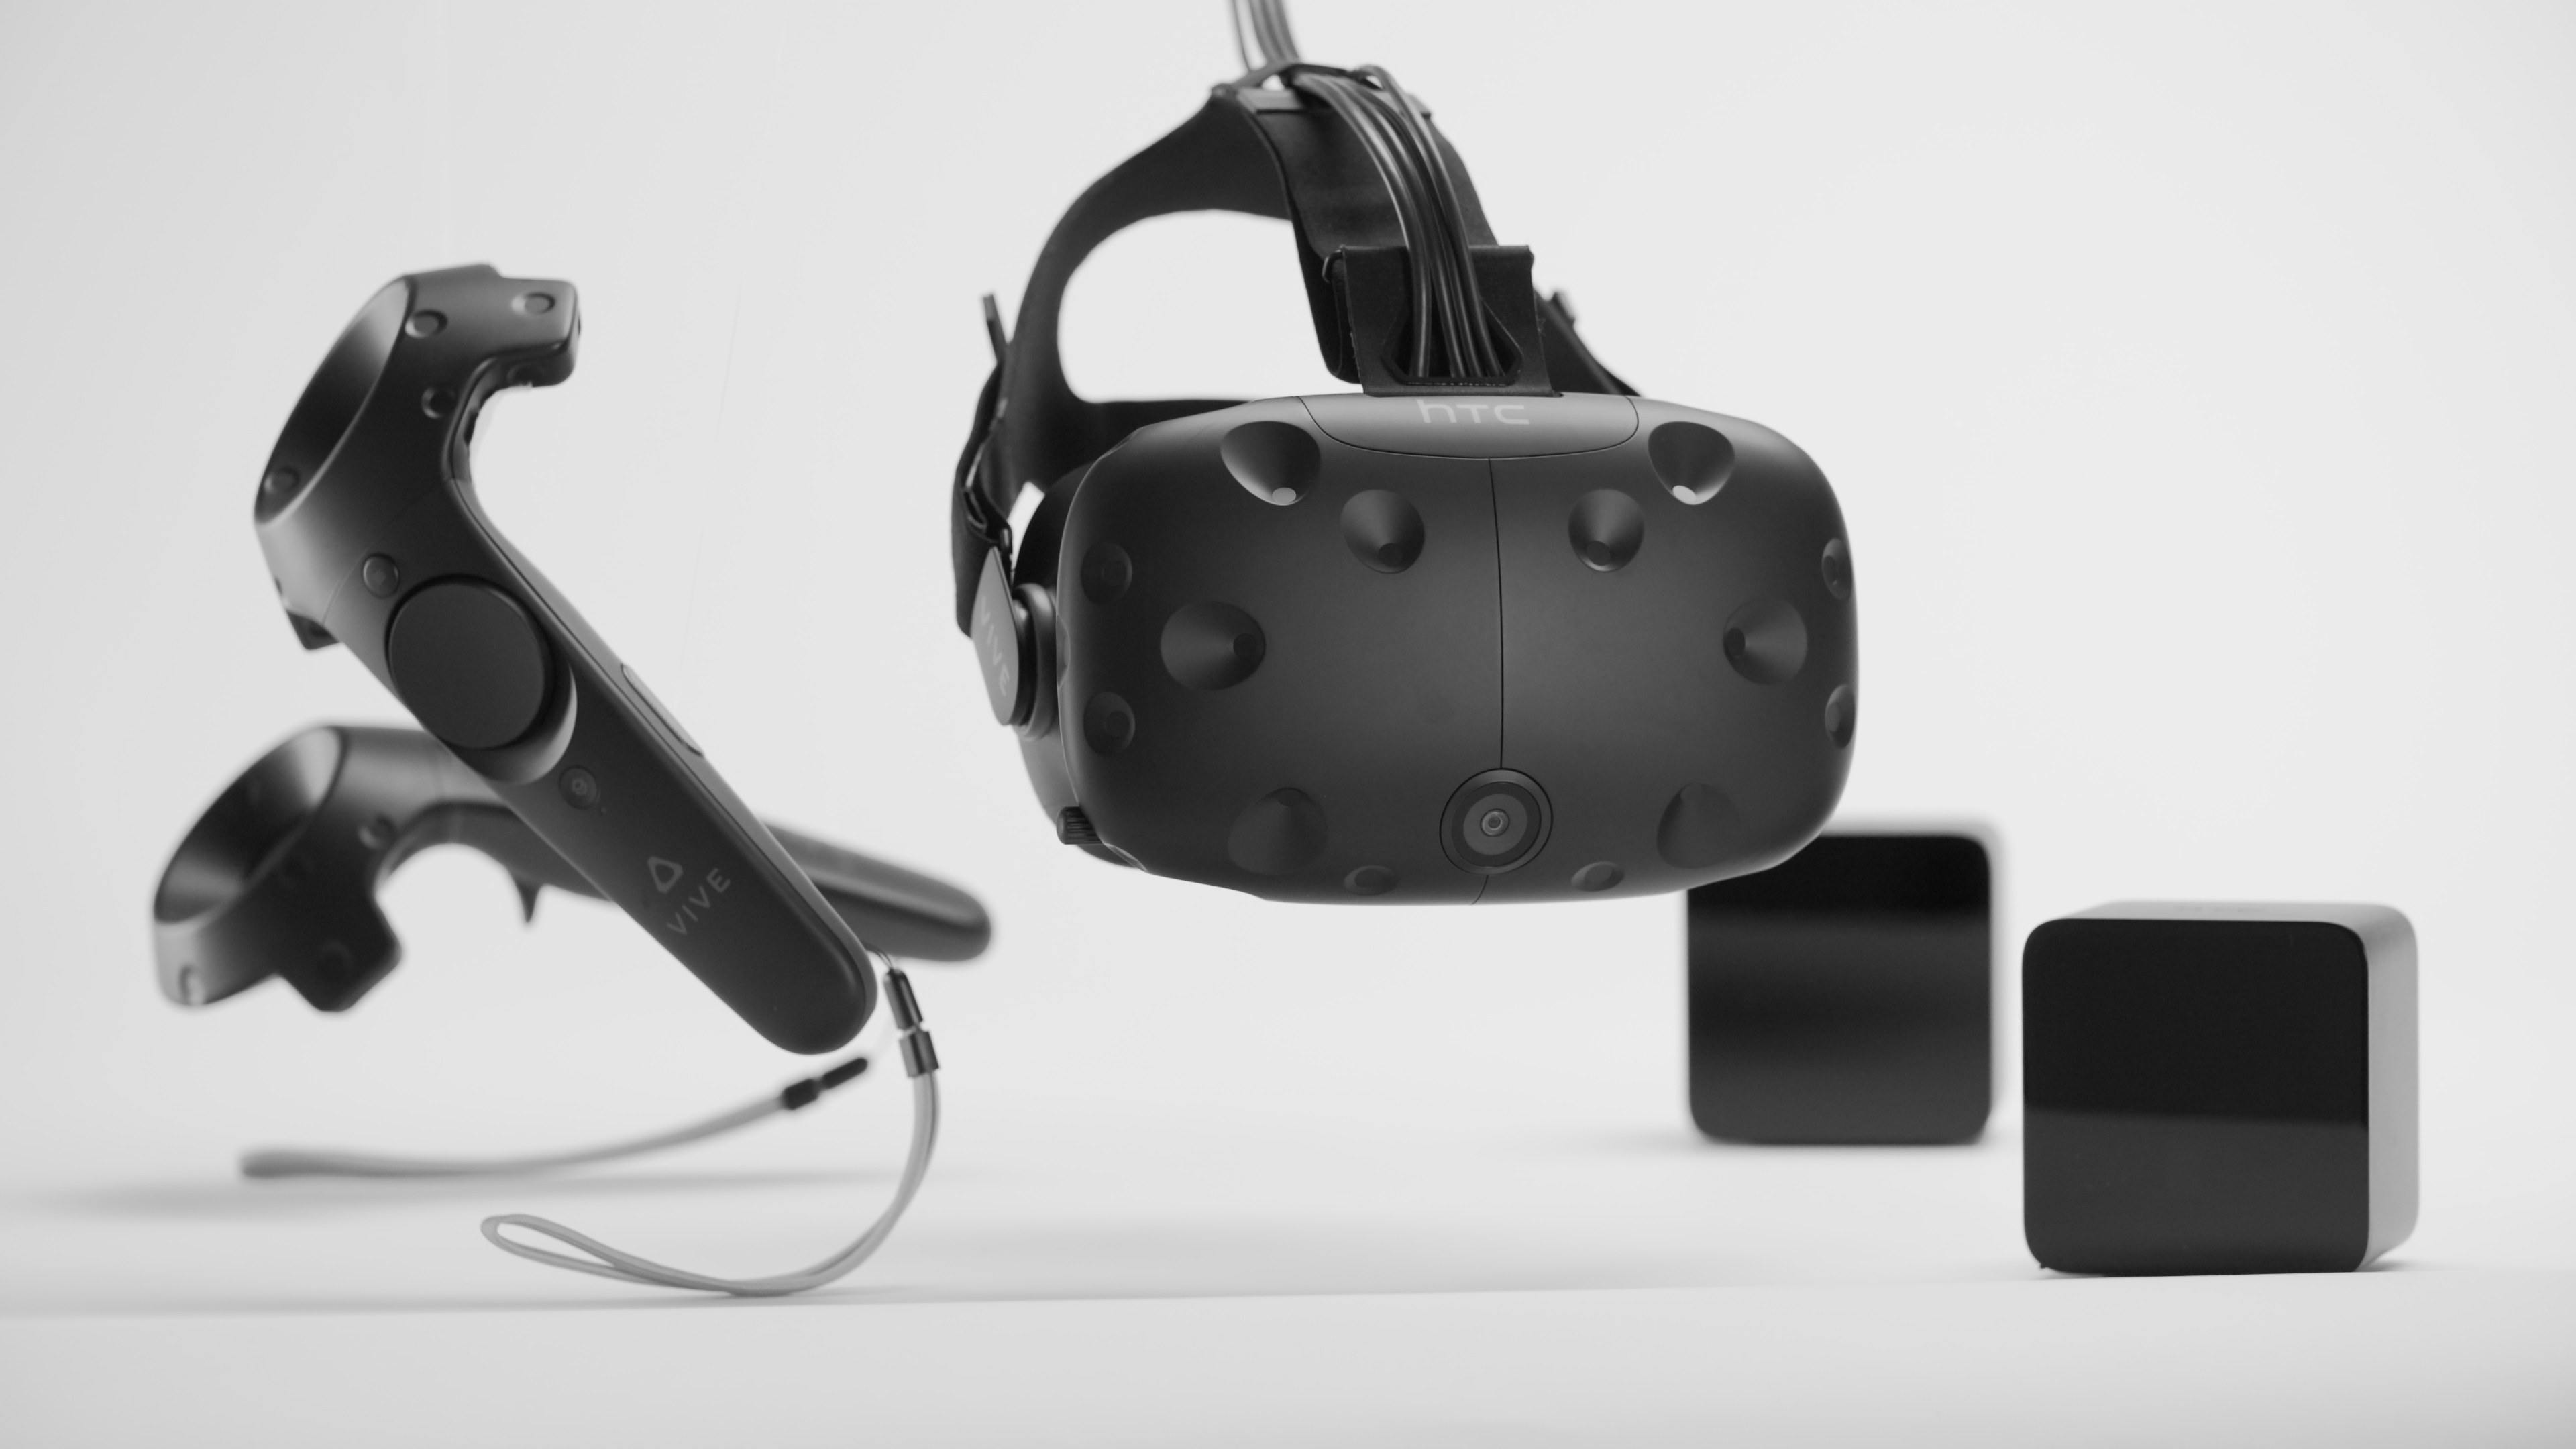
\includegraphics[width=\textwidth]{background/fig/vive-cne-featured.jpg}
		\caption{HTC Vive Test Gear Set}
		\label{fig:vive}
	\end{subfigure}
	\begin{subfigure}[b]{0.4\textwidth}
		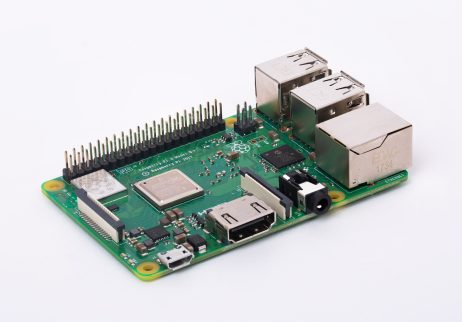
\includegraphics[width=\textwidth]{background/fig/pi.jpg}
		\caption{Raspberry Pi 3 Model B+}
		\label{fig:camera}
	\end{subfigure}        
	\caption{External equipment}\label{fig:T34}
\end{figure}
With the use of a standalone build from official websites, the video processing Library is meant to modify video streams from a camera before they get received by Unity. 
This unusual approach served as a temporary fix, to avoid an issue which requires a complete recompile of entire FFmpeg-autogen Library, used by Unity Engine as a prefab.\\[1pt]
This report will present progress in 4 agile-based development stages: Investigation, Integration, Design and Testing. \\
If scope and aim to set a foundation and growing interest in AR technology to attract business leaders use this opportunity to cover VR full potential~\cite{jain_know_2017}, the project will lead to breaking through experience.\\[1pt]
Concerning practical usage, one of the goals is to demonstrate possible usage and entertain one of mixed reality.
Based on~\cite{abishur_prakash_augmented_2018}, the AR takes place in manufacturing, healthcare and defence to improve overall human performance.
Following his understanding, it may be used as a training program to prepare a human face for real difficulties.
Relying on first-hand experience, taking the example of Tank-34, which requires 2-4 human pilots to operate, the idea may set a solid foundation for other possible extensions.
Achieving similar real tank driving results in an in-game engine may require people with far higher experience.
Game designing is one of the limitations, which passed through this report early.
Similar designer problems are left to more experienced developers.
The overall idea of implementation relates to a morally old video game, Battlefield 3, created by DICE.
This game provided the closest simulation of the tank commander back in 2012, when a player acted as a gunner of Primary and Secondary weapons, occasionally taking a look inside driver and Mechanic operations.
Figure~\ref{fig:BF3} represents such transitions on each subfigure.
\begin{figure}[H]
	\centering
	\begin{subfigure}[b]{0.4\textwidth}
		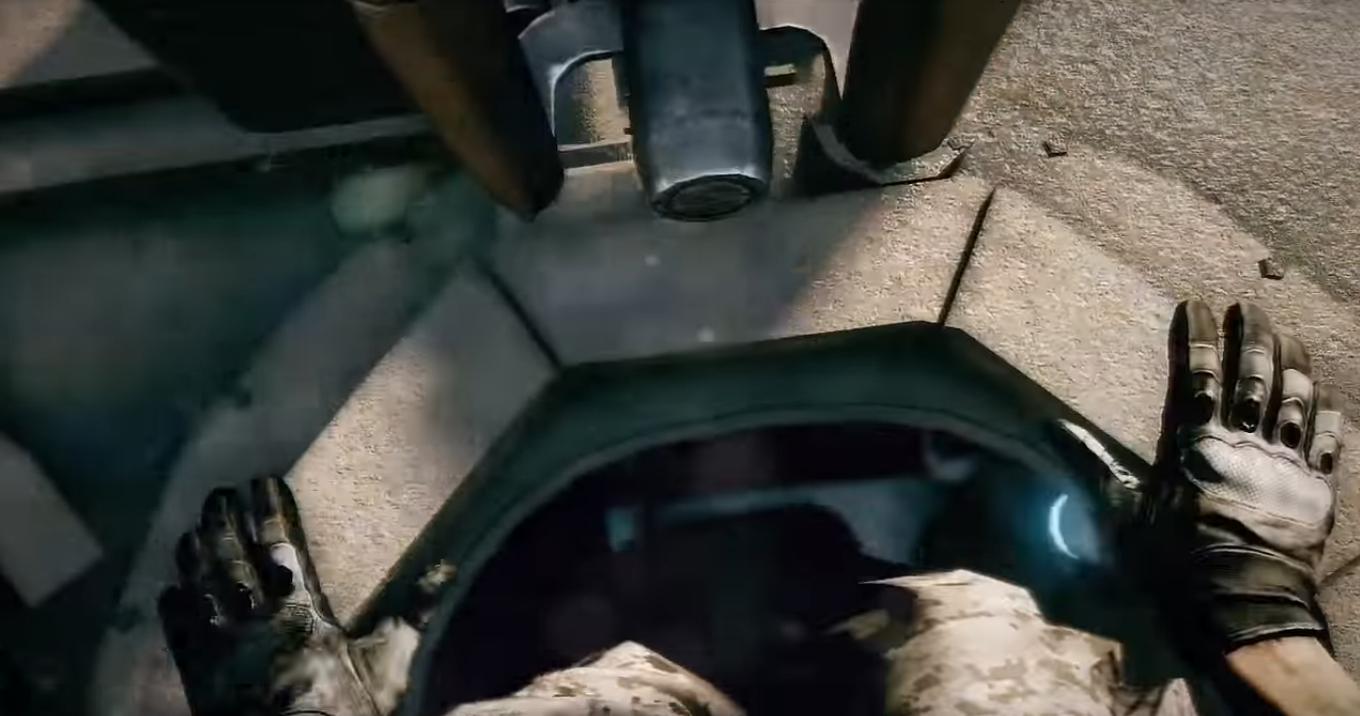
\includegraphics[width=\linewidth]{background/fig/BF3-1.png}
		\caption{Changing view between tank and turret}
		\label{fig:inside}
	\end{subfigure}
	\begin{subfigure}[b]{0.4\textwidth}
		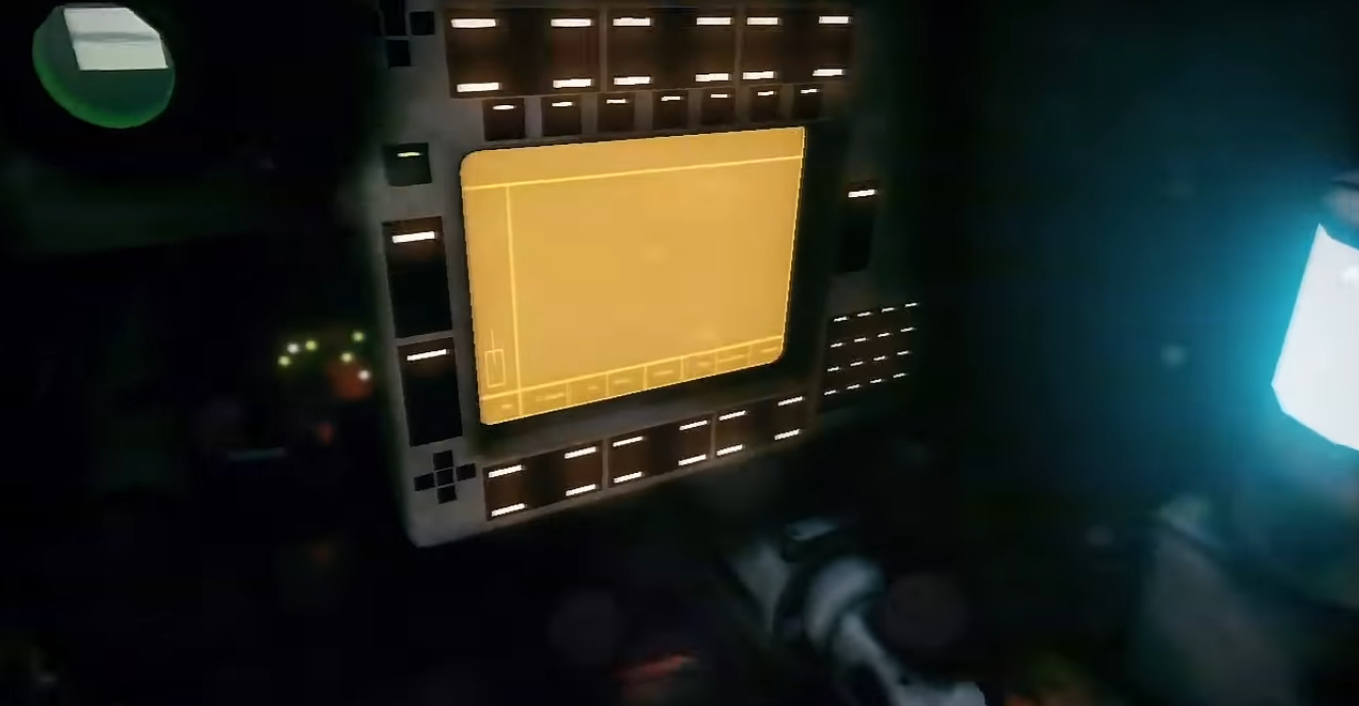
\includegraphics[width=\linewidth]{background/fig/BF3-2.png}
		\caption{Entering Tank view screen}
		\label{fig:tank}
	\end{subfigure}
	\caption{Battlefield 3 Tank gameplay footage}\label{fig:BF3}
\end{figure}
The approach can also provide excellent teaching opportunities by eliminating danger and the need for extra instruction from humans by replacing the instructor with AI~\cite{abishur_prakash_augmented_2018}.
Steam~\cite{steam_workshop_tanks_2018} game Library consists of similar games or similar tank simulations, but so far, none ever tried combined with Augmented Reality\\[1pt]
However, The good thing is that the Mech-Warfare delivered a similar experience but from the top view, as in strategic or isometric games~\cite{mech-warfare_mech-warfare_2015}.
Combine such experience with similar games as Arktica.1 by 4A Games~\footnote{Ukraine company, creators of Metro 2033 and Last Light. Now they developed Metro Exodus using RTX technology}, subfigure~\ref{fig:mech}.
\begin{figure}[H]
	\centering
	\begin{subfigure}[b]{0.4\textwidth}
		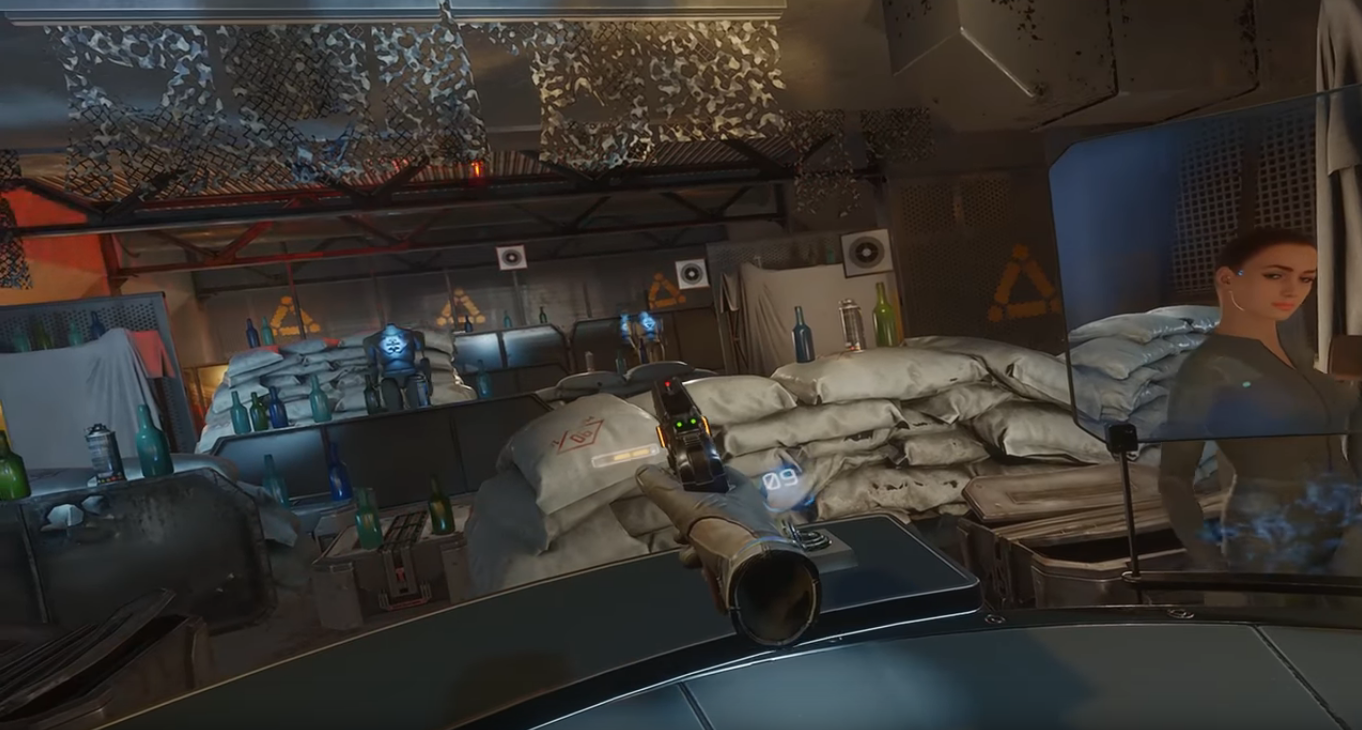
\includegraphics[width=\linewidth]{background/fig/Arkticak1.png}
		\caption{Arktica.1 Gameplay footage}
		\label{fig:OculusArc}
	\end{subfigure}
	\begin{subfigure}[b]{0.4\textwidth}
		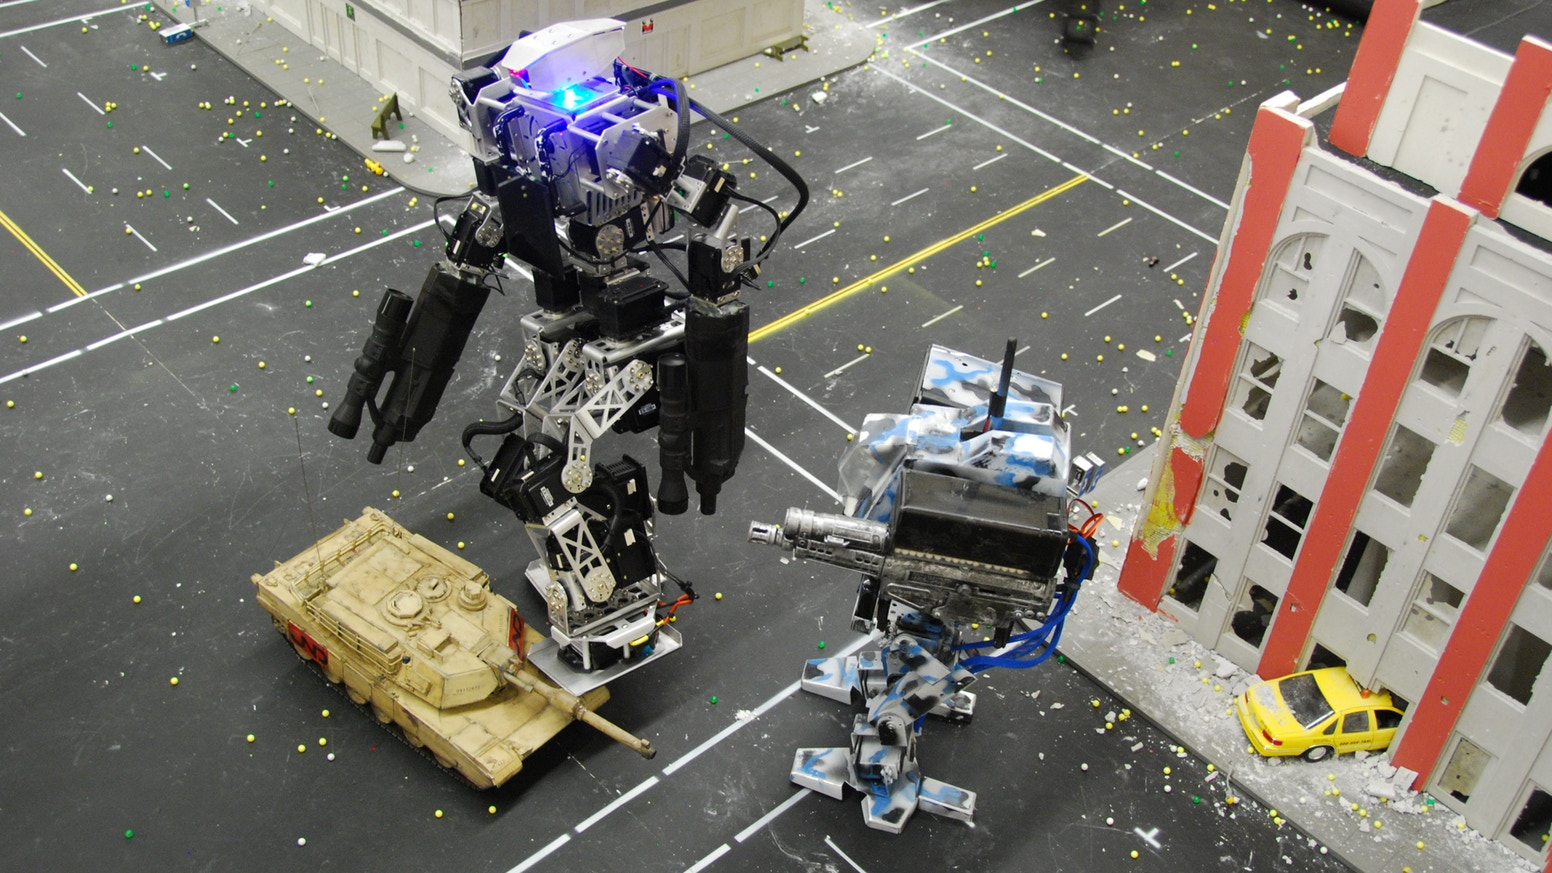
\includegraphics[width=\linewidth]{background/fig/mech.jpg}
		\caption{Mech-Warfare Game play}
		\label{fig:mech}
	\end{subfigure}        
	\caption{Example from Arktica.1 and Mech-Warfare}\label{fig:play-exampl}
\end{figure}
Nevertheless, the project has a solid background to follow and a good chance of producing satisfactory results.
%%%%%%%%%%%%%%%%%%%%%%%%%%%%%%%%%%%%%%%%%%%%%%%%%%%%%%%%%%%%%
%This served as a temporary fix, to avoid an issue which requires a complete recompile of entire ffmpeg-autogen Library, used by Unity Engine as a prefab.\\
% \begin{wrapfigure}{r}{0.5\textwidth}
% 	\begin{center}
% 		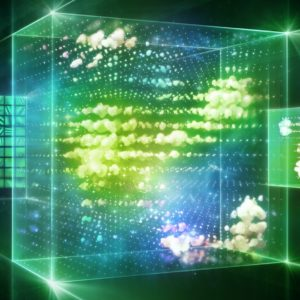
\includegraphics[width=0.35\textwidth]{background/fig/cuda.jpg}
% 	\end{center}
% 	\caption{CUDA AI programming}
% 	\label{fig:cuda}
% \end{wrapfigure}
%The usage of CUDA~\cite{noauthor_cuda_2012} efficiency is only meant to be discovered and applied. The application of additional techniques like RAMCache - ASUS technology of memory management~\cite{asus_introduction_2017}, multi-threading and proper video streaming codec methods will be left for the remaining time or stored for future work.\\
\newpage
\begin{landscape}
    A conceptual diagram on the next page is meant to bring an overview of the structure of the entire project and how all components are linked to each other.
	\begin{figure}[H]%[htbp]
        \centering
        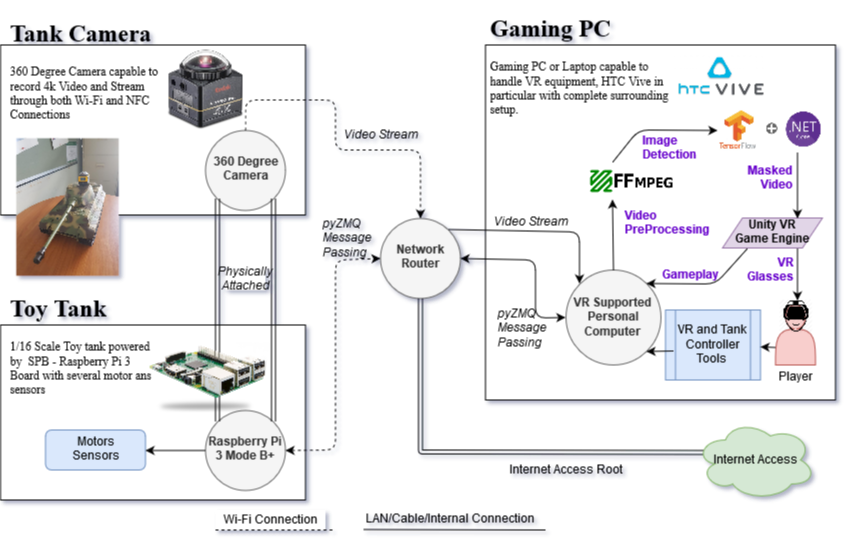
\includegraphics[width=0.8\linewidth]{background/fig/ConceptDiagram.png}
        \caption{A top-down view on the project}
    \end{figure}
\end{landscape}
